\chapter{Contributions}

\section{Analyse technique}

Notre objectif est de déformer l'écran pour fournir à l'utilisateur un meilleur confort visuel. 
L'année précédente j'ai réalisé un prototype de déformation d'image avec le système d'exploitation Windows. Ce prototype était une application développée en C++ Opengl, étant capable de capturer l'affichage des applications exécutées sous Windows et également le bureau, d'afficher ces rendus et de les déformer via un shader.
Cependant ce prototype nous a permis d'observer les limites de développer ce projet sous un système d'exploitation fermé (sans accès au code source). En effet, capturer les images, comme fait le prototype, est gourmand pour la VRAM (~200 Mbits pour une image 4k) et ne permet pas d'obtenir de bonnes performances (~50 fps). De plus l'API de Windows est limité dans notre cas d'utilisation ce qui ne nous permet pas d'accéder et de modifier librement tout ce qui est effectué au niveau du gestionnaire de fenêtres, nommé WDDM sous Windows. Aucun test n'a été effectué sous Mac OS X puisque nous ne disposons d'aucune machine exécutant ce système d'exploitation. Notre choix de système d'exploitation s'est donc orienté vers le système GNU/Linux qui est un OS libre et open source ce qui nous permettra potentiellement de modifier chaque composant du système.

Pour effectuer la déformation plusieurs solutions techniques s'offrent à nous.

\subsection{Modification de librairies graphiques}

L'idée d'effectuer la déformation graphique à partir de la librairie graphique n'est pas viable. D'une part, toutes les librairies graphiques sont en constante évolution. Modifier le code source de ces librairies serait une tâche pénible et devrait être tenu à jour en fonction des nouvelles spécificités de chaque nouvelle version. Maintenir le code source serait donc une tâche impossible. De plus cette solution ne serait pas applicable pour l'ensemble de notre écran. Imaginons que l'on modifie la librairie GTK, si une application QT est exécutée elle ne bénéficiera pas de la déformation que l'on applique avec les autres applications GTK.

Modifier les librairies serait donc une tâche fastidieuse, complexe et non générique pour obtenir une déformation sur l'ensemble d'un seul et même système d'exploitation.

Une autre solution peut-être plus générique serait de hacker les serveurs d'affichages.

\subsection{Hack des serveurs d'affichages}

Sous GNU/Linux il existe principalement un serveur d'affichage nommé X. X Window System, X11 ou encore X est un environnement graphique de type fenêtré qui gère l'interaction homme-machine par l'écran, la souris et le clavier de certains ordinateurs en réseau. Il est souvent appelé X Window à ne pas confondre avec x windows. C'est le système standard ouvert d'interaction graphique avec l'utilisateur sur les systèmes UNIX (Linux, BSD, etc.). X utilise une architecture client serveur, dont la partie serveur est responsable d'effectuer le rendu graphique qui sera envoyé à l'écran. Cette solution technologique se rapproche de ce que nous souhaitons mettre en place avec la déformation globale de l'écran. Cependant X est un serveur d'affichage datant d'une trentaine d'années dont le code source est une accumulation de patchs et est aujourd'hui difficile à maintenir. Faire la déformation au niveau de X serait donc une tâche complexe en matière de développement. De plus l'ensemble de la communauté GNU/Linux élabore un nouveau protocole d'affichage nommé Wayland qui permettra dans les années, voire mois, à venir de supprimer X pour un système plus moderne. 

Wayland est encore jeune (première version datante de 2008) et n'est seulement qu'un protocole de serveur d'affichage. Aujourd'hui Wayland est déjà fonctionnel dans certains gestionnaires de bureau, comme Gnome ou encore KDE (fonctionnel depuis juin 2015). Wayland inclut une rétro-compatibilité en gérant les applications utilisant les librairies de X, ce qui le rend complètement opérationnel avec toutes les applications GNU/Linux. Wayland fournit un moyen pour les gestionnaires de fenêtres composites de communiquer directement avec les applications graphiques ainsi que le materiel video. Les applications effectuent leurs rendus graphiques dans une mémoire tampon qui leur sont dédiés et le gestionnaire de fenêtres composites, devenu serveur d’affichage, se charge de les assembler pour construire l’image à afficher sur l’écran. Wayland propose donc une architecture plus simple et efficace que ce que propose le serveur d’affichage X. 

Toutefois, modifier le code source de ces serveurs d'affichage est une tâche complexe et une solution plus simple reste à modifier les environnements de bureau.

\subsection{GNU/Linux Gnome et Fragment Shader}

Gnome est environnement de bureau énormément utilisé sous le système GNU/Linux et est dans la plupart des distributions l'environnement de bureau proposé par défaut. De plus il est l'un des rares environnements de bureau à avoir déjà implémenté Wayland. L'implémentation de Wayland est importante dans notre cas car avec le prototype réalisé sous Windows, un problème lié à la déformation est apparu. Il existe une différence entre ce qui est affiché à l'écran et les inputs envoyés au système. Cette question sera traitée plus tard dans ce rapport mais Wayland est une solution à X puisque la gestion des inputs est séparée et connue par tout le système et donc une modification des inputs serait donc plus facile avec Wayland.

Gnome est implémenté avec la librairie Clutter qui est une bibliothèque logicielle permettant la création rapide d'interfaces graphiques visuellement riches et animées. C'est un projet libre (licence GNU LGPL) et multiplate-forme. Clutter est soutenu commercialement par OpenedHand, société depuis rachetée par Intel, et par une communauté open source de plus en plus grande. Clutter utilise OpenGL et permet donc l'utilisation des shaders. Reprendre le fragment shader de déformation du prototype et l'appliquer à l'ensemble de notre bureau est donc une méthode réalisable rapidement.

En effet, dans le pipeline d'OpenGL l'une des dernières manipulations effectuées avant l'envoi des données à l'écran est l'application du fragment shader, voire figure \ref{fig:glPipeline}.

\begin{figure}[h!]
	\center	
	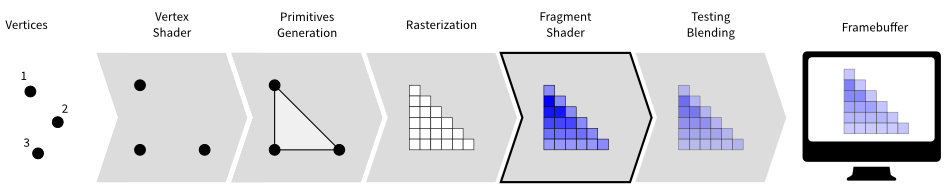
\includegraphics[scale=0.6]{image/glPipeline.png}
	\caption{Schéma du pipeline OpenGL}
	\label{fig:glPipeline}
\end{figure}

Lors du prototype précédemment réalisé sous Windows, la déformation d'image était assuré par un fragment shader. Un fragment shader a pour but de calculer la couleur de chaque pixel individuellement. Il prend ainsi en entrée les données de chaque pixel de l'image (position, coordonnées de texture, couleur) et renvoie la couleur de celui-ci. C'est donc l'une des dernières étapes réalisées par le GPU avant d'envoyer les données à l'écran. De plus les shaders étant des opérations extrêmement rapides, la déformation d'image via fragment shader n'aura aucun impact sur le framerate global.

La popularité de Gnome, son avancé technologique avec Wayland, ainsi que son architecture avec des librairies telles que Clutter ou Mutter en font un choix judicieux pour assurer la pérennité du projet. La distribution GNU/Linux utilisé sera donc Fedora 22, distribution connue et utilisée par les développeurs de Gnome.




















\section{Tracking utilisateur}

\subsection{Libgina}

Pour réaliser la partie tracking utilisateur, le framework Libgina a été utilisé. Libgina est un outil développé par Nicolas Bremard, doctorant de l'équipe MINT. Libgina est un framework qui consiste à fournir un écosystème permettant de facilement ajouter un ou des périphériques de capture utilisateur, d'effectuer des traitements sur ces données, de définir des gestes à reconnaître, de propager les données, etc.

\subsection{Kinect}

Kinect est l’outil développé par l’entreprise PrimeSense et popularisé par Microsoft avec la Xbox 360. Il s’agit d’une caméra permettant de contrôler avec son corps, ou par commande vocale des applications, jeux, etc. Prime-Sense  fournit des codes samples permettant d’utiliser les outils de détection de mouvements, de squelettes et de communication vocale. La détection du squelette sera utilisée et plus particulièrement la détection de la tête et des mains pour pouvoir interagir face à l'écran géant et permettre à notre fonction de déformation de calculer la déformation nécessaire compte tenue de la position de l'utilisateur face à l'écran.

\begin{figure}[!h]
	\center	
	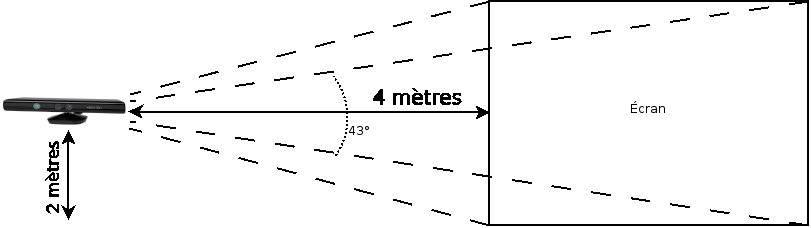
\includegraphics[scale=0.5]{image/kinectScreen.png}
	\caption{Configuration de la Kinect face à l'écran}
	\label{fig:kinectScreen}
\end{figure}

L'utilisation de la Kinect est pertinente puisqu’il s’agit d’un outil grand public, à faible coût et qui peut être facilement mis en place dans le cadre de grands écrans dans des lieux publics.

La Kinect dans notre configuration nécessite d'être positionné face à l'écran à une distance de quatre mètres, une position en hauteur de 2 mètres et une inclinaison de -15\degres pour traquer l'utilisateur face à l'écran, voire figure \ref{fig:kinectScreen}. Dans cette configuration, l'écran occupe en largeur et en hauteur l'image obtenue de la Kinect.

Dans libgina, une partie KinectGenerator va récupérer les données du squelette de l'utilisateur pour ensuite permettre un traitement sur ces mêmes données et les transmettre à la fonction de déformation.

Cependant la Kinect est un outil datant de 2010 avec une qualité d'image d'acquisition médiocre ce qui ne permet pas une grande précision dans la détection exacte de l'utilisateur dûe aux problèmes d'occlusions. Du bruit est également présent sur les données de positions calculées ce qui rend la déformation visuellement instable et donc visuellement inconfortable pour l'utilisateur.

Pour pallier le problème du bruit produit par la Kinect le One Euro Filter \cite{oneeuro} a été utilisé. Le One Euro filter est un algorithme permettant de filtrer un tracé. Il est développé par INRIA et l’implémentation est disponible en \textit{JavaScript} ou encore en \textit{C++}. C'est un filtre passe-bas, c’est-à-dire que les hautes fréquences sont éliminées. Cela permet ainsi d'éliminer les tremblements des jointures du squelette. Cependant le One Euro Filter introduit une latence entre le déplacement et la déformation de l'écran ce qui ne peut être une solution finale envisageable.

\subsection{Optitrack}

Les optitrack sont des caméras infrarouges produites par le groupe NaturalPoint. Elles sont connues pour être utilisées pour faire de la capture de mouvement pour le cinéma ou les jeux vidéo. Le grand atout de cette technologie est la précision de tracking approchant l'ordre du millimètre, la rapidité des caméras allant jusqu'à 250 images/s, ainsi que la facilité d'utilisation et de calibration du logiciel MotiveBody calculant la position des trackers en fonction de la position des différentes caméras. 
Pour l'anamorphose dynamique nous avons configuré deux trackers que l'utilisateur devra porter lors de l'utilisation. Une constellation sur la tête, qui permettra de déterminer la position et l'orientation de la tête face à l'écran et une constellation sur la main droite, qui permettra à l'utilisateur de faire du pointage.
Les positions et orientations des différentes constellations sont ensuite envoyées sur le réseau en utilisant le protocole VRPN. VRPN (Virtual-Reality Peripheral Network) est une bibliothèque libre fournissant une interface transparente entre une application de réalité virtuelle tournant sur une machine et des dispositifs physiques (trackers, wand, haptic device) connectés à d'autres machines d'un réseau.

Dans Libgina un VRPNGenerator a été créé pour permettre de récupérer la position et l'orientation des différentes constellations. Cette classe pourra être réutilisée dans le futur pour fournir une base logicielle aux personnes souhaitant travailler avec Libgina et le protocole VRPN. 

\subsection{Transmission des données utilisateur}

Une fois les données utilisateurs récupérées de la Kinect ou des Optitrack, des traitements sont effectués sur ces données dans Libgina. Une normalisation des données est effectuée. Nos données \textit{x,y,z}, de la tête et des mains, vont varier entre 0 et 1 en fonction de la position de l'utilisateur dans un cube de quatre mètres de profondeur, deux mètres de haut et quatre mètres de large. Ce cube représente l'espace d'interaction que l'on a défini en fonction de la taille de l'écran et de la profondeur avec lequel l'utilisateur peut interagir avec l'écran.

Une fois les traitements effectués les nouvelles données sont transmisses aux composants gnomes-shell par protocole UDP aux ports 2021 et 2022. 





















\section{Anamorphose dynamique}

Ce projet se base sur l’anamorphose dynamique de Solina et al. \cite{Schmidt:2013:SEP:2470654.2466227}. Notre objectif est donc d'apporter le concept d'anamorphose dynamique mono-utilisateur aux systèmes d'exploitation moderne, dans notre cas la distribution GNU/Linux Fedora 22 qui embarque l'écosystème Gnome disposant de la compatibilité Wayland. Wayland est un protocole de communication qui dans les années futures va remplacer le serveur graphique X.org qui est aujourd'hui le plus utilisé par les systèmes d'exploitation Linux.

\subsection{Définition de la formule de déformation}


Pour déterminer comment faire la déformation, nous nous sommes basé sur ce qui a été présenté dans l'état de l'art concernant l'acuité visuelle de l'être humain. Comme dit précédemment l'être humain à une vision binoculaire de 120\degres ($\simeq$ 60\degres par oeil). Pour déterminer l'équation nous avons utilisé les fonctions trigonométriques, voir \ref{fig:trigo}.

\begin{figure}[h!]
	\center	
	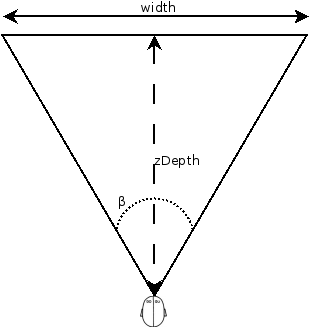
\includegraphics[scale=0.3]{image/anamorphose_formule.png}
	\caption{Schéma trigonométrique de la formule de déformation d'image}
	\label{fig:trigo}
\end{figure}

\begin{align*}
  \tan(\beta)&=\frac{width/2}{zDepth}&
  \beta&=\arctan(\frac{width/2}{zDepth})&
\end{align*}

La distance à partir de laquelle l'effet de déformation apparaîtra est de  XXX mètres.

Avant, l'effet n'est pas nécessaire car l'écran ne couvre pas le champ visuel binoculaire. Une fois entrée dans cet intervalle avec l'écran, la fonction de déformation sera paramétrée avec le Zdepth qui variera entre 0 et 1. 1 signifiant les XXX mètres et 0 le contact avec l'écran. Pour garder une certaine cohérence avec le rendu visuel la fonction de déformation n'atteindra jamais la valeur 0. En effet si Zdepth atteint 0 cela correspond à afficher un pixel à l'écran. Or, même au contact de l'écran, afficher un pixel apporterait un rendu visuel inadapté. La valeur zDepth sera donc limitée à XXX.

Le rendu visuel sera un étirement de la zone de l'écran à afficher sur la même résolution, voire \ref{fig:deformationImage}.

\begin{figure}[h!]
	\center	
	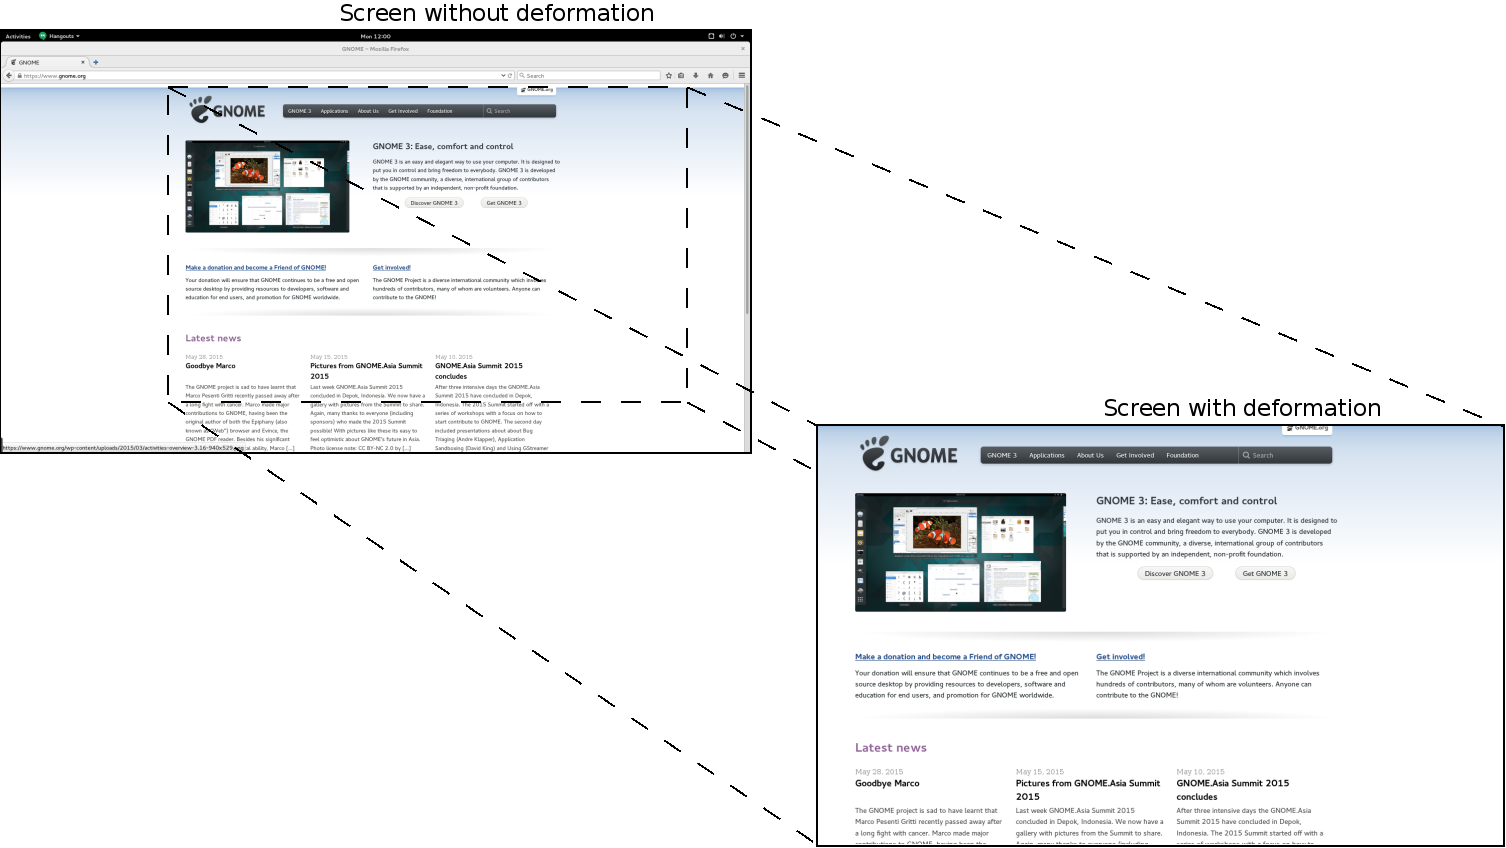
\includegraphics[scale=0.25]{image/deformationImage.png}
	\caption{Schéma de déformation de l'image}
	\label{fig:deformationImage}
\end{figure}

Cette partie de la déformation étant faite il a fallut l'intégrer dans un système d'exploitation. Le gestionnaire d'affichage Gnomme Shell a été sélectionné pour appliquer la déformation d'image pour le système GNU/Linux.


\subsection{Extension Gnome-Shell}

Comme expliqué précédemment, pour appliquer l’effet de déformation sur l’ensemble de l’écran et non uniquement à une application, l’environnement Linux/Gnome a été retenu. L’ensemble des explications, modifications du code qui suivent sont liés à l’environnement graphique Gnome.

Dans un premier temps, une tentative d’implémentation pour déformer l’image a été réalisé en extension Gnome-Shell. Gnome-Shell étant le coeur de l'interface graphique de l'environnement de bureau Gnome.

Le problème est que malgré toutes les possibilités offertes par le système d’extension de Gnome-Shell, nous sommes passé à une solution plus bas niveau. En effet, pour appliquer une déformation de l’affichage il faut écrire du code C avec Clutter pour appliquer des changements dans le fragment shader qui permettent de dessiner l’interface graphique. Changer le shader d'affichage dans une extension Gnome est réalisable mais non adapté à l'architecture que nous voulions implémenter. De plus, la librairie Clutter fournit des objets dont l'objectif est d'appliquer des effets visuels aux éléments de dessin.

\subsection{Modification du code source de Gnome-Shell}
Gnome-Shell est implémenté en Javascript mais fait appel à des librairies écrites en C, qui elles effectuent des modifications et des appels bas niveau. Voir la figure ~\ref{fig:anamorphoseSchema} globale des modifications qui ont étés apportés à Gnome-Shell.

\begin{figure}[!h]
	\center	
	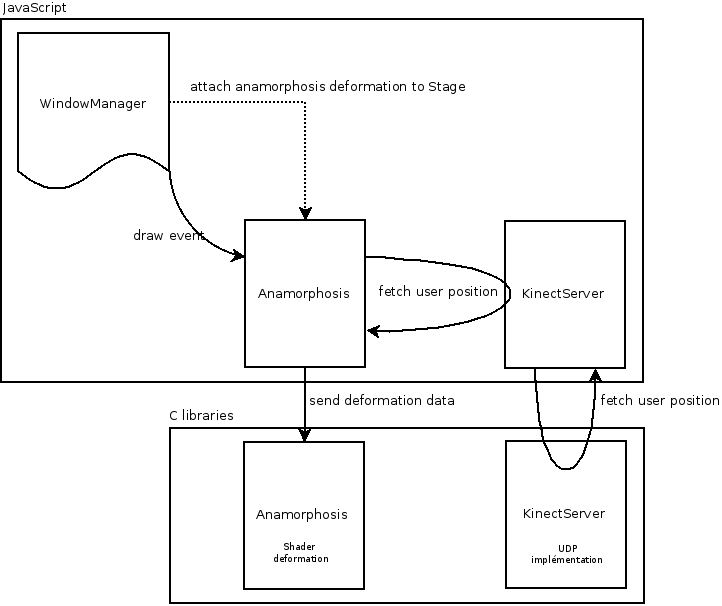
\includegraphics[scale=0.5]{image/anamorphose_schema.png}
	\caption{Schéma d'implémentation de l'anamorphose dans Gnome-Shell}
	\label{fig:anamorphoseSchema}
\end{figure}

Des ClutterEffects sont des objets Clutter permettant d'appliquer un effet à d'autres objets Clutter. Les ClutterEffects permettent donc de modifier le shader d'affichage. Le Stage représente la racine des éléments graphiques dans Clutter. Lorsque l'on applique une déformation au Stage l'ensemble de l’écran est affecté par l'effet présent dans le ClutterEffects. 

\begin{figure}[!h]
	\center	
	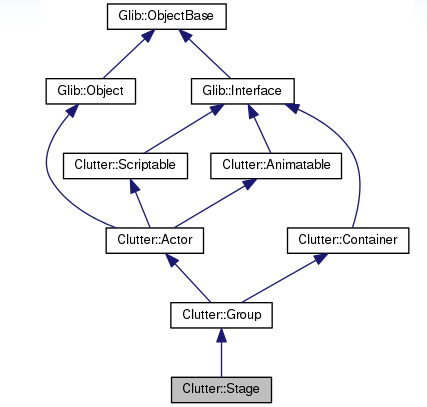
\includegraphics[scale=0.4]{image/clutterStage.png}
	\caption{Vue de l'héritage de ClutterStage dans Clutter}
	\label{fig:clutterStage}
\end{figure}

Dans Clutter, il existe le type ClutterActor qui est un élément de base du graphe de scène, voire la figure ~\ref{fig:clutterStage}. La racine du graphe de la scene représente l’ensemble de l’écran et est appelé Stage. Ce Stage est de type ClutterStage et hérite de ClutterActor. Il est possible d’ajouter aux ClutterActors des ClutterEffects. ClutterEffect est une classe fournissant une API pour créer des effets qui seront appliqués aux ClutterActor et qui permettent de modifier la manière dont le ClutterActor est dessiné sans avoir à modifier l’actor.

Voici comment est appliqué le ClutterEffect au Stage en Javascript :

\begin{lstlisting}[language=JavaScript]
global.stage.add_effect_with_name("ActorAnamorphosis", new Shell.AnamorphosisEffect());
\end{lstlisting}

Le ClutterEffect que nous avons créé consiste à ajouter du comportement au fragment shader utilisé par défaut pour appliquer l’effet d’anamorphose dynamique. Celui-ci implémente la fonction de déformation citée précédemment. Le code source est disponible en annexe de ce rapport, voire \annexe{sec:SCDefImage}






























\section{Déformation des évènements système pour l'anamorphose dynamique}

\subsection{Concept}

La gestion de la souris est particulière. Le curseur est dessiné par la carte graphique et non par le système d’exploitation. Par conséquent, quand la déformation est appliquée au système cela n’a aucun impact sur le curseur de la souris, aussi bien en matière de rendu qu’en matière de position virtuelle.

En d'autres termes, la souris se comporte comme si l'écran n'était pas déformé et sa position en pixel correspond au pixel de la texture de l'écran non déformé. 

\begin{figure}[!h]
	\center	
	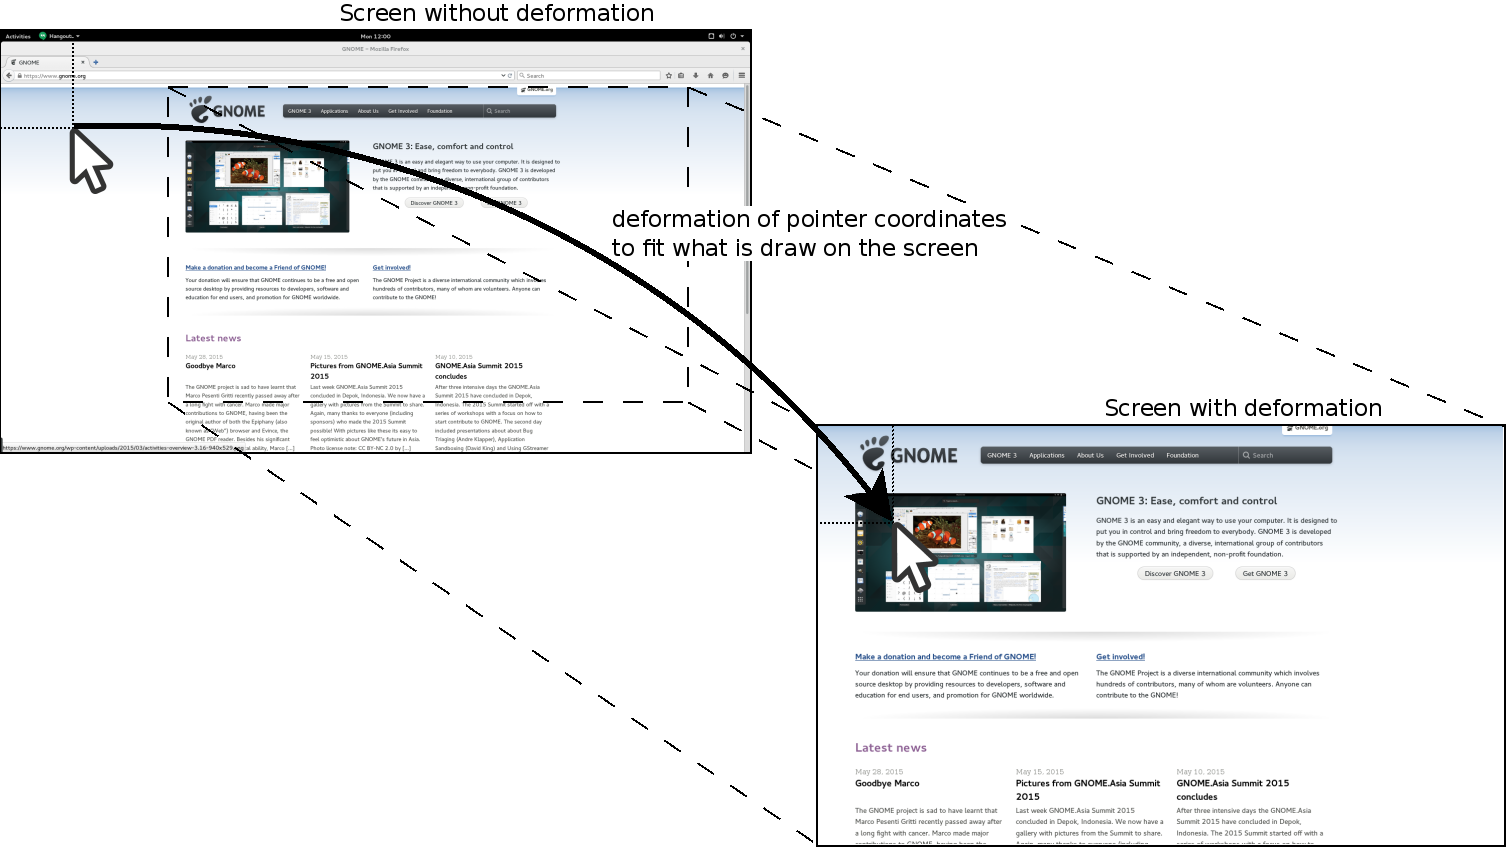
\includegraphics[scale=0.25]{image/deformationCurseur.png}
	\caption{Schéma de déformation du curseur}
	\label{fig:deformationCurseur}
\end{figure}

Dans la figure~\ref{fig:deformationCurseur} on schématise l'idée de la déformation du curseur qui est mise en place lorsque l'écran est déformé. On modifie dans la librairie Clutter la position renvoyée de la souris pour faire correspondre son emplacement réel à ce qui est dessiné sur l'écran.

\subsection{Implémentation }

Pour implémenter cette déformation deux solutions logicielles se sont proposées. 

\subsubsection{Serveur d'affichage X}

Comme présenté précédemment X est le serveur d'affichage le plus utilisé des GNU/Linux. Le serveur d'affichage X a pour responsabilité, en plus de devoir faire le rendu visuel, de gérer tous les évènements d'entrée. Il s'occupe donc du clavier et de la souris et les propage aux applications et au gestionnaire de fenêtres si ces derniers les réclament. Ce qui autrement dit, signifie que l'environnement de bureau n'a aucune idée d'où se situe la souris s'il ne réclame pas sa position. Imaginons qu'une application soit ouverte et que ma souris interagit avec cette application, seulement l'application a connaissance de la position de la souris et non le gestionnaire de fenêtres.

Avec cette gestion des événements d'entrée il est donc impossible de modifier la position de la souris en fonction de la déformation visuelle sans avoir à modifier X. Comme présenté plus haut dans ce rapport, X est un serveur d'affichage datant d'une trentaine d'années dont le code source est une accumulation de patchs et est aujourd'hui difficile à maintenir. Suite à cette analyse, s'offre une solution qui tend à remplacer le serveur X sur les futures distributions Linux, Wayland.

\subsubsection{Wayland}
Wayland contrairement à X laisse d'autres librairies gérer les entrées système. 
Libinput est la librairie qui s'occupe de gérer les entrées système et a pour objectif de transmettre ces informations au Wayland compositor, qui pour Gnome et Mutter. Cette implémentation avec Mutter Clutter et Gnome permet à l'ensemble de l'environnement de bureau de connaître la position de la souris.
Le couple Wayland/Gnome est donc fort intéressant car contrairement à X, tous les événements souris passent par une fonction (voir listing \ref{lst::clutterInput}) de la librairie Clutter y compris si une fenêtre demande le focus souris. 

\begin{lstlisting}[caption={Fonction clutter fournissant les coordonnées x y des périphérique d'entrée}\label{lst::clutterInput}, language=C++]
gboolean
clutter_input_device_get_coords (ClutterInputDevice *device,
						     ClutterEventSequence *sequence, 
						     ClutterPoint         *point);
\end{lstlisting}

La fonction permettant la déformation est la même fonction que pour la déformation de l'image. Les coordonnés pixels du fragment shader correspondent içi aux coordonnées \textit{(x,y)} du périphérique d'entrée. 

Le code de déformation des coordonnées est disponible en annexe de ce rapport, voire \annexe{sec:SCDefInputs}.




























\section{Magnifying-glass déformation}

Conscient que l'anamorphose dynamique ne peut être utilisé dans tout les cas d'utilisation il nous a fallut une autre méthode pour augmenter le confort visuel à distance. Comme dit précédemment, l'anamorphose dynamique s'active à partir de XXXX mètres. Si nous souhaitons utiliser l'écran géant à une distance plus élevée il faut pouvoir rendre visible des details de l'écran qui ne sont pas ou peu visible avec une densité d'affichage aussi élevée.

Pour répondre au problème de lisibilité à distance sur l'écran géant, une loupe autrement appelée magnifying glass en anglais a été proposé comme solution au problème. Deux types de loupe sont intéressants dans notre contexte, une dite contextuelle qui permettra d'afficher l'écran avec un effet fisheye, l'autre sera une loupe de lecture.

Dans les deux loupes étudiées nous avons voulu garder une vision de l'écran globale et non ce que propose actuellement Windows ou Gnome-Shell avec des loupes qui occupent une partie de l'écran et dont l'interaction souris se fait via une exploration de l'espace de travail, comme présenté dans l'état de l'art. 


\subsection{Loupe contextuelle}

La loupe contextuelle permet une distorsion de l'écran qui utilise l'effet fisheye. Pour réaliser cette déformation d'image nous avons du trouver une fonction mathématique réalisant un effet fisheye. Voici la formule utilisée pour réaliser la loupe contextuelle :

\begin{align*}
  deformation=(-depth/radius)*distance + (depth/(radius*radius))*distance^{2}&
\end{align*}

\textit{Depth} est un paramètre faisant varier le paramètre de zoom, en photographie cela pourrait correspondre à la focale. \textit{radius} correspond à la taille en pourcentage de la loupe par rapport à l'écran. Et \textit{distance} correspond à la distance entre le pixel dessiné et le centre de la loupe. Un aperçu de la fonction est visible, voire figure \ref{fig:loupeContexteFormule}, avec pour paramètre un \textit{radius} de 0.4. 

\begin{figure}[!h]
	\center	
	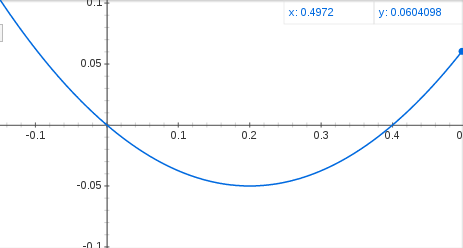
\includegraphics[scale=0.5]{image/loupeContexteFormule.png}
	\caption{Aperçu de la loupe contextuelle}
	\label{fig:loupeContexteFormule}
\end{figure}


Pour implémenter cette loupe, le ClutterEffect développé pour la déformation d'image a été reprit. Le shader a été modifié pour permettre d'utiliser la formule correspondant à la loupe contextuelle. La loupe a été implémenté en C avec le ClutterEffect et une autre partie envoyant la position de la souris a été écrite Javascript. Dans la cas d'utilisation de la loupe nous avons utilisé le système d'extension Gnome-Shell. Une fois l'extension activée il suffit de cliquer sur l'icône de la loupe, présente dans la barre des tâches, pour activer ou désactiver l'effet de la loupe.

Voici un aperçu de la loupe contextuelle, voire figure \ref{fig:loupeContexte}
Une démonstration ainsi que le code source sont disponibles sur le site shadertoy \url{https://www.shadertoy.com/view/llsSz7}
\begin{figure}[!h]
	\center	
	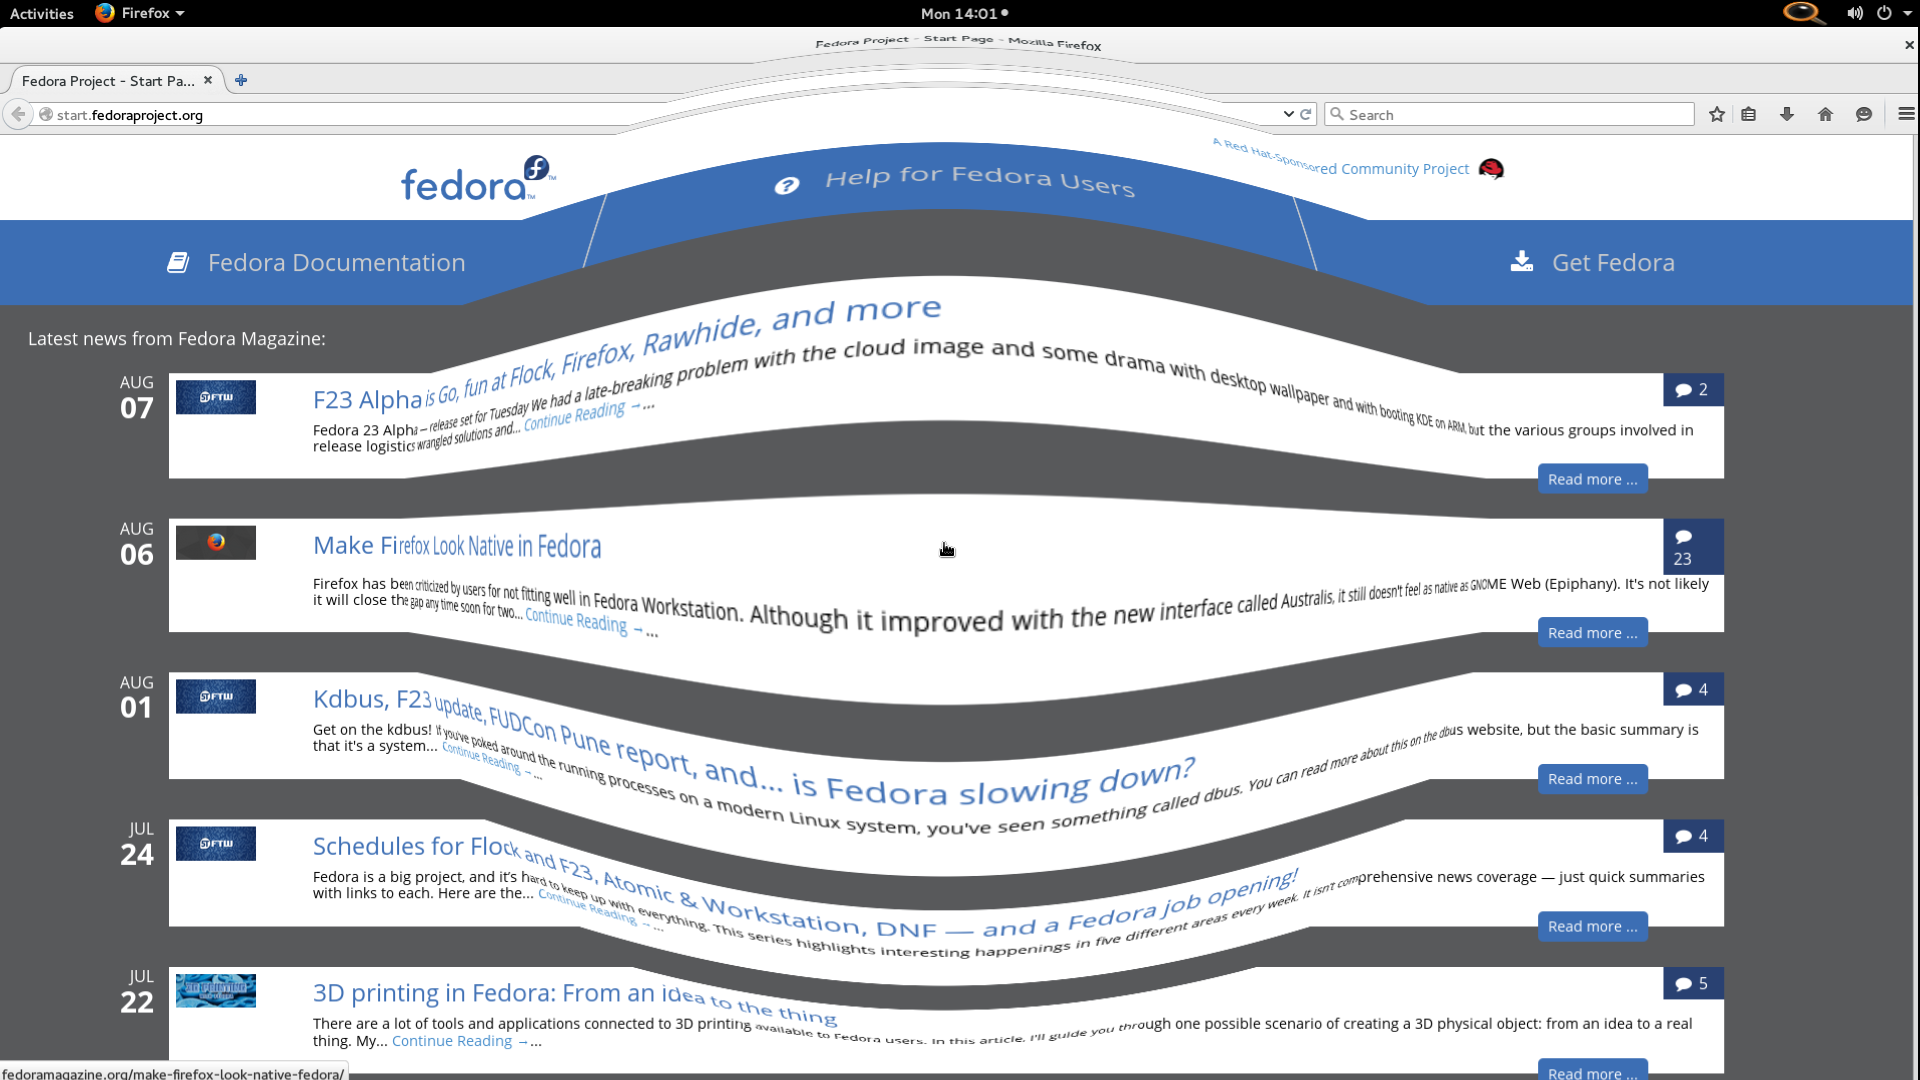
\includegraphics[scale=0.25]{image/loupeContexte.png}
	\caption{Aperçu de la loupe contextuelle}
	\label{fig:loupeContexte}
\end{figure}

\subsection{Loupe de lecture}

Concernant la loupe de lecture, cette dernière n'a pas été implémenté due à un manque de temps. Cependant son implémentation est relativement rapide puisqu'il s'agit simplement d'écrire un shader que l'on intègre dans des fichiers similaires à ce que l'on a fait dans la déformation dynamique ou encore avec la loupe. L'ensemble des outils présentés précédemment sont génériques et peuvent accueillir de nouvelles formules de déformation.